%
% Main document
% ===========================================================================
% This is part of the document "Project documentation template".
% Authors: brd3, kaa1
%

%---------------------------------------------------------------------------
\documentclass[
	a4paper,					% paper format
	10pt,							% fontsize
	twoside,					% double-sided
	openright,				% begin new chapter on right side
	notitlepage,			% use no standard title page
	parskip=half,			% set paragraph skip to half of a line
]{scrreprt}					% KOMA-script report
%---------------------------------------------------------------------------

\raggedbottom
\KOMAoptions{cleardoublepage=plain}			% Add header and footer on blank pages


% Load Standard Packages:
%---------------------------------------------------------------------------
\usepackage[standard-baselineskips]{cmbright}

\usepackage[ngerman,english]{babel}										% english hyphenation
%\usepackage[latin1]{inputenc}  							% Unix/Linux - load extended character set (ISO 8859-1)
\usepackage[ansinew]{inputenc}  							% Windows - load extended character set (ISO 8859-1)
\usepackage[T1]{fontenc}											% hyphenation of words with �,� and �
\usepackage{textcomp}													% additional symbols
\usepackage{ae}																% better resolution of Type1-Fonts 
\usepackage{fancyhdr}													% simple manipulation of header and footer 
\usepackage{etoolbox}													% color manipulation of header and footer
\usepackage{graphicx}                      		% integration of images
\usepackage{float}														% floating objects
\usepackage{caption}													% for captions of figures and tables
\usepackage{booktabs}													% package for nicer tables
\usepackage{tocvsec2}
\usepackage{lipsum}
% provides means of controlling the sectional numbering
%---------------------------------------------------------------------------

% Load Math Packages
%---------------------------------------------------------------------------
\usepackage{amsmath}                    	   	% various features to facilitate writing math formulas
\usepackage{amsthm}                       	 	% enhanced version of latex's newtheorem
\usepackage{amsfonts}                      		% set of miscellaneous TeX fonts that augment the standard CM
\usepackage{amssymb}													% mathematical special characters
\usepackage{exscale}													% mathematical size corresponds to textsize
%---------------------------------------------------------------------------

% Package to facilitate placement of boxes at absolute positions
%---------------------------------------------------------------------------
\usepackage[absolute]{textpos}
\setlength{\TPHorizModule}{1mm}
\setlength{\TPVertModule}{1mm}
%---------------------------------------------------------------------------					
			
% Definition of Colors
%---------------------------------------------------------------------------
\RequirePackage{color}                          % Color (not xcolor!)
\definecolor{linkblue}{rgb}{0,0,0.8}            % Standard
\definecolor{darkblue}{rgb}{0,0.08,0.45}        % Dark blue
\definecolor{bfhgrey}{rgb}{0.41,0.49,0.57}      % BFH grey
%\definecolor{linkcolor}{rgb}{0,0,0.8}     			% Blue for the web- and cd-version!
\definecolor{linkcolor}{rgb}{0,0,0}        			% Black for the print-version!
%---------------------------------------------------------------------------

% Hyperref Package (Create links in a pdf)
%---------------------------------------------------------------------------
\usepackage[
	pdftex,ngerman,bookmarks,plainpages=false,pdfpagelabels,
	backref = {false},										% No index backreference
	colorlinks = {true},                  % Color links in a PDF
	hypertexnames = {true},               % no failures "same page(i)"
	bookmarksopen = {true},               % opens the bar on the left side
	bookmarksopenlevel = {0},             % depth of opened bookmarks
	pdftitle = {Template fuer Bachelor Thesis},	   	% PDF-property
	pdfauthor = {brd3},        					  % PDF-property
	pdfsubject = {LaTeX Template},        % PDF-property
	linkcolor = {linkcolor},              % Color of Links
	citecolor = {linkcolor},              % Color of Cite-Links
	urlcolor = {linkcolor},               % Color of URLs
]{hyperref}
%---------------------------------------------------------------------------
% Set up page dimension
%---------------------------------------------------------------------------
\usepackage{geometry}
\geometry{
	a4paper,
	left=28mm,
	right=15mm,
	top=30mm,
	headheight=20mm,
	headsep=10mm,
	textheight=242mm,
	footskip=15mm
}
%---------------------------------------------------------------------------

% Makeindex Package
%---------------------------------------------------------------------------
\usepackage{makeidx}                         		% To produce index
\makeindex                                    	% Index-Initialisation
%---------------------------------------------------------------------------

% Glossary Package
%---------------------------------------------------------------------------
% the glossaries package uses makeindex
% if you use TeXnicCenter do the following steps:
%  - Goto "Ausgabeprofile definieren" (ctrl + F7)
%  - Select the profile "LaTeX => PDF"
%  - Add in register "Nachbearbeitung" a new "Postprozessoren" point named Glossar
%  - Select makeindex.exe in the field "Anwendung" ( ..\MiKTeX x.x\miktex\bin\makeindex.exe )
%  - Add this [ -s "%tm.ist" -t "%tm.glg" -o "%tm.gls" "%tm.glo" ] in the field "Argumente"
%
% for futher informations go to http://ewus.de/tipp-1029.html
%---------------------------------------------------------------------------
\usepackage[acronym,nonumberlist]{glossaries}
\makeglossaries
\newglossaryentry{Accelerometer}{name={Accelerometer},description={A sensor which detect acceleration}}

\newglossaryentry{Gyroscope}{name={Gyroscope},description={A sensor which detects orientation and angular velocity \cite{Gyroscop33:online}}}

\newglossaryentry{ESP32}{name={ESP32},description={Low cost, low power, microcontroller by espressif \cite{ESP32Ove27:online}}}

\newglossaryentry{Microcontroller}{name={Microcontroller},description={A small computer on a single chip}}


\newglossaryentry{SD}{name={Secure Digital},description={A memory card standard}}

\newglossaryentry{RTC}{name={RTC},description={Real Time Clock - Computer clock that keeps track of time \cite{Realtime16:online}}}


\newglossaryentry{MPU6050}{name={MPU6050},description={Six Axis gyroscope and acceleremoter motion tracking device \cite{MPU6050T29:online}}}


\newglossaryentry{IoT}{name={Internet of Things},description={Connected computing devices and digital machines}}

\newglossaryentry{lipo battery}{name={lithium polymer battery},description={Energy storage technology}}

\newglossaryentry{MQTT}{name={MQ Telemetry Transport},description={Machine to machine connectivity protocol \cite{MQTT46:online}}}

\newglossaryentry{JSON}{name={JavaScript Object Notation},description={"A lightweight data interchange format" \cite{JSON31:online}}}

\newglossaryentry{Protobuf}{name={Protocol Buffers},description={"Protocol buffers are Google's language-neutral, platform-neutral, extensible mechanism for serializing structured data" \cite{Protocol99:online}}}

\newglossaryentry{CSV}{name={Comma Separated Values},description={Text file that contains structured data}}


\newglossaryentry{MVC}{name={Model-View-Controller},description={Design pattern used to decouple user-interface (view), data (model), and application logic (controller)" \cite{ASPNETMV81:online}}}


\newglossaryentry{Power BI}{name={Power BI},description={A data visualsiation tool from Microsoft \cite{PowerBIM60:online}}}


\newglossaryentry{Python}{name={Python},description={High level programming language \cite{Welcomet27:online}}}

\newacronym{mqtt}{MQTT}{MQ Telemetry Transport}
 
\newacronym{iot}{IoT}{Internet of Things}

\newacronym{protobuff}{Protobuf}{Protocol Buffer}

\newacronym{json}{JSON}{JavaScript Object Notation}

\newacronym{csv}{CSV}{Comma Separated Values}

\newacronym{sd}{SD}{Secure digital}


\newacronym{rtc}{RTC}{Real Time Clock}
%---------------------------------------------------------------------------

% Intro:
%---------------------------------------------------------------------------

\usepackage{wrapfig, blindtext}
\usepackage{gensymb}
\usepackage{listings}
\begin{document}                              	% Start Document
\settocdepth{section}														% Set depth of toc
\pagenumbering{roman}	
 

%---------------------------------------------------------------------------

\providecommand{\heading}{Position Yourself}		%  Insert Title of Thesis here					% Titel der Arbeit aus Datei titel.tex lesen
\providecommand{\versionnumber}{3.0}			%  Hier die aktuelle Versionsnummer eingeben
\providecommand{\versiondate}{11.06.2019}		%  Hier das Datum der aktuellen Version eingeben				% Versionsnummer und -datum aus Datei version.tex lesen

% Set up header and footer
%---------------------------------------------------------------------------
\makeatletter
\patchcmd{\@fancyhead}{\rlap}{\color{bfhgrey}\rlap}{}{}		% new color of header
\patchcmd{\@fancyfoot}{\rlap}{\color{bfhgrey}\rlap}{}{}		% new color of footer
\makeatother

\fancyhf{}																		% clean all fields
\fancypagestyle{plain}{												% new definition of plain style	
	\fancyfoot[OR,EL]{\footnotesize \thepage} 	% footer right part --> page number
	\fancyfoot[OL,ER]{\footnotesize \heading, Version \versionnumber, \versiondate}	% footer even page left part 
}
\renewcommand{\chaptermark}[1]{\markboth{\thechapter.  #1}{}}
\renewcommand{\headrulewidth}{0pt}				% no header stripline
\renewcommand{\footrulewidth}{0pt} 				% no bottom stripline

\pagestyle{plain}
%---------------------------------------------------------------------------
% Title Page and Abstract
%---------------------------------------------------------------------------
%\include{leader/frontpage_without_picture}		% activate for frontpage without picture
%
% Project documentation template
% ===========================================================================
% This is part of the document "Project documentation template".
% Authors: brd3, kaa1
%

\begin{titlepage}


% BFH-Logo absolute placed at (28,12) on A4 and picture (16:9 or 15cm x 8.5cm)
% Actually not a realy satisfactory solution but working.
%---------------------------------------------------------------------------
\setlength{\unitlength}{1mm}
\begin{textblock}{20}[0,0](28,12)
	
\includegraphics[scale=1.0]{images/BFH_Logo_B.png}
\end{textblock}

\begin{textblock}{154}(28,48)
	\begin{picture}(150,2)
		\put(0,0){\color{bfhgrey}\rule{150mm}{2mm}}
	\end{picture}
\end{textblock}

\begin{textblock}{150}[0,0](28,50)
	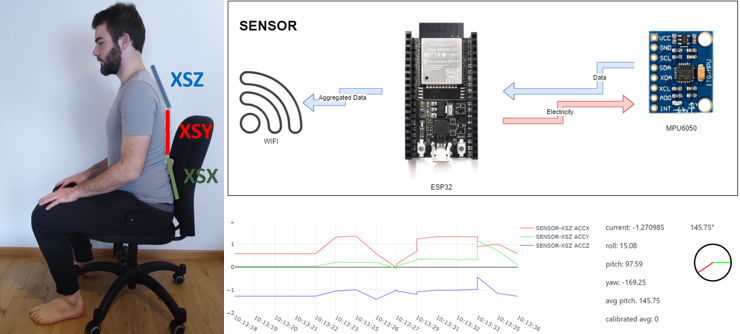
\includegraphics[width=\linewidth]{images/TitlePicture.png}
\end{textblock}

\begin{textblock}{154}(28,117)
	\begin{picture}(150,2)
		\put(0,0){\color{bfhgrey}\rule{150mm}{2mm}}
	\end{picture}
\end{textblock}
\color{black}

% Institution / titel / subtitel / authors / experts:
%---------------------------------------------------------------------------
\begin{flushleft}

\vspace*{115mm}

\fontsize{26pt}{28pt}\selectfont 
\heading				\\							% Read heading from file leader/title.tex
\vspace{2mm}

\fontsize{16pt}{20pt}\selectfont\vspace{0.3em}
A wearable IoT solution			\\				% Insert subheading
\vspace{5mm}

\fontsize{10pt}{12pt}\selectfont
\textbf{} \\		% Insert text
\vspace{3mm}

% Abstract (eingeben):
%---------------------------------------------------------------------------
\begin{textblock}{150}(28,190)
\fontsize{10pt}{12pt}\selectfont
Creating a prototype with modern IoT comoponents and topical knowhow to track and improve posture.
\end{textblock}

\begin{textblock}{150}(28,225)
\fontsize{10pt}{17pt}\selectfont
\begin{tabbing}
xxxxxxxxxxxxxxx\=xxxxxxxxxxxxxxxxxxxxxxxxxxxxxxxxxxxxxxxxxxxxxxx \kill
Authors:		\> Gabriel Frischknecht		\\					% insert names
Tutor:	\> Prof. Dr.~Reto Koenig		\\
Expert:	\> Prof. Dr.~Torsten Braun		\\% insert names
Date:			\> \versiondate					\\							% read from file leader/version.tex
\end{tabbing}

\end{textblock}
\end{flushleft}

\begin{textblock}{150}(28,280)
\noindent 
\color{bfhgrey}\fontsize{9pt}{10pt}\selectfont
Berner Fachhochschule | Haute \'ecole sp\'ecialis\'ee bernoise | Bern University of Applied Sciences
\color{black}\selectfont
\end{textblock}


\end{titlepage}

%
% ===========================================================================
% EOF
%
		% activate for frontpage with picture
\section{Abstract}



\setcounter{page}{1}


\cleardoublepage
%---------------------------------------------------------------------------

% Table of contents
%---------------------------------------------------------------------------
\tableofcontents
\cleardoublepage
%---------------------------------------------------------------------------

% Main part:
%---------------------------------------------------------------------------
\pagenumbering{arabic}
\renewcommand\thefigure{\arabic{figure}}

\addcontentsline{toc}{chapter}{Acknowledgements}
\chapter*{Acknowledgements}
\label{chap:Acknowledgements}
\renewcommand{\thesection}{\arabic{section}}
\setcounter{section}{0}

First and foremost, I would like to thank my tutor, Prof. Dr. Reto Koenig for his guidance and support during my work.
I further thank Prof. Dr. Torsten Braun for supervising my thesis in the role of the expert.

Finally, I would like to thank my partner, MSc cand. BSc Valerie Zumbrunnen, who supported me during this thesis, not only emotionally but also with her in depth know-how and experience as a physiotherapist she contributed greatly to the outcome of this thesis.


\addcontentsline{toc}{chapter}{Introduction}
\chapter*{Introduction}
\label{chap:Introduction}
\renewcommand{\thesection}{\arabic{section}}
\setcounter{section}{0}

The long-term goal of this Project was first defined in 2017 and has been refined ever since. First and for most, the goal is to create a simple and cheap device(s) which can measure and improve posture. Additional it should all be open source and recreatable. Besides posture, the goal is also to offer a way to improve balance. 
With the idea of improving balance also comes a much larger goal which might not even be achievable. The solutions should be able to find application in the medicinal field, however this seams to be nearly impossible due to the complexity and restrictions in this field. 

Therefore I decided to split the long term goal into smaller steps which should be achievable one by one individually. During this thesis I will try to achieve the following:

Firstly I will need to find out how many Sensors are needed to get an understanding of the users Gait and Position. To Achieve this I will also need to find a way to visualise or interpret the data I am collecting.

\addcontentsline{toc}{chapter}{First Attempts}
\chapter*{The first attempts}
\label{chap:The first attempts}
\renewcommand{\thesection}{\arabic{section}}
\setcounter{section}{0}

I thought that the interesting part of this project, is the simplicity and low-technicality. However the implementation turned out to be much more complex than expected. This attempt unfortunately was not accompanied with the expected success.

\section{The Android App}

The very first approach to the posture "problem" was an android App. The standard android phone offers all necessary actors and sensors and is therefore a great test environment: 
\begin{enumerate}
    \item \gls{Accelerometer} - Detects acceleration
    \item \gls{Gyroscope} - Detect orientation and angular velocity \cite{Gyroscop33:online}
    \item Vibrators
    \item Storage
\end{enumerate}

This means it was possible to get live data and calculate position and pitch in real time. Thanks to the built in vibration units, it was also possible to vibrate when a threshold was reached. With enough Android development know-how, this implementation is achievable swiftly and did work as expected.

The usability was not great and it did not feel very professional. The phone had to be held and placed near the chest or back to work. This would mean the first use case, improving the sitting position, was not achievable without holding or attaching the phone to the user and not using your phone while at work. Therefore the android app idea was quickly put aside. Since, for now at least, it does not offer what is desired.

\newpage
\section{The IoT Solution}

The next plan was to create a simple \acrshort{iot} solution (\gls{IoT}).Which I thought could be achieved by combining actors, sensors and a bit of code. However it was not as easy as expected, since the sensors and positional data is rather complex. 

The code is running on a \gls{microcontroller}, an ESP 32, specifically an ESP32 WEMOS Lolin V1.0.0. The very specific version is quite important. I will go further in depth into why, in the \textbf{difficulties}.

The \gls{ESP32} was chosen, since it offers everything you can imagine. It has a built in Bluetooth module, Wifi module and supports nearly all modern Android libraries and components. On top of that the ESP32 is cheap. It can be bought from Swiss sellers for about 10-15 CHF. It can also be imported via aliexpress.com for as low as 2-5 CH. The delivery time however, can take up to 2 months. Therefore, I considered it to be a perfect contestant for this project. 

Additionally, to the microcontroller a few more items are needed to fullfill the needed requirements. A Gyroscope, an Accelerometer, Vibrators, A Real Time Clock (\acrshort{rtc}) and a \acrshort{sd}-Card (\gls{SD}) module. The \gls{RTC} is needed since we want to log the measured values, and to analyse or visualise these logs, a time-stamp is necessary. 

All modules I have used, are used in so called breakout boards. These make the testing and development easier by offering pin-out and -in to enable swift testing. Without breakout boards the parts would be a lot smaller, however, not suitable for a first prototype since it would complicate the development process.

\subsection{The Gyroscope and Accelerometer}

After investigating, which modules are available on the market, I have decided to use the 
\gls{MPU6050} Chip since it is widely used and is documented very well. 

\begin{wrapfigure}[11]{l}{0.3\textwidth}
  \begin{center}
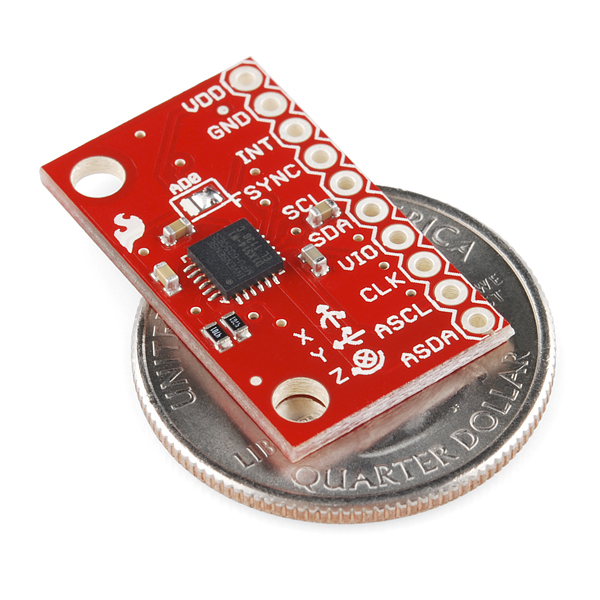
\includegraphics[width=0.3\textwidth]{images/MPU_6050.jpg}

  \end{center}
  \caption{MPU6050}
  \label{fig:MPU6050}
\end{wrapfigure}

The MPU6050 communicates via the \textbf{Wire library} and has a built in thermometer, accelerometer and gyroscope. The module is also really tiny even if it is a breakout board.
Without the breakout board this sensor would be reduced to the black square since in the picture (\ref{fig:MPU6050}).

The MPU6050 is documented very precisely which was a great help during development and made it quite easy to get the correct values. This Chip would also offer the possibility to perform some calculations directly on the Chip. Unfortunately, this part of the MPU6050 is very obfuscated. It would increase the complexity vastly without offering real benefits. This however, might be something, which will be considered in further development steps of this project.

The MPU has a very high complexity and it was quite a challenge to understand all the data, that the device provides. Especially reading the data showed to be much harder than expected. However, after some research and a lot of testing, it turned out to be much easier than firstly expected, since I was able to read the gravity which affects the accelerometer.
Currently only the values of the accelerometer are used to determine the position and sense the direction in which the user is leaning. This might be a bit to simple for the ergonomic use case, however, it is a good starting point and no technical modification are needed to get additional values.

The code for the calculation and reading of values is quite complex and really long. Therefore I will not put any code snippets in this sections since they would not provide the desired benefits to the reader. However, the whole source code will be available in my git repository. \cite{GF3RGabr46:online} \cite{TDKAttra32:online}

\newpage

\subsection{The Wire library}

To communicate with the MPU6050 and the RTC, SD Card module the wire library is necessary. With this library the communication and data exchange over only two cables (SDA Serial Data Line, SCL Serial Clock Lin) is made possible. Both modules communicate through these cables. These are located at port 21 and portvis 22 on the ESP32. The communication protocol is quite simple, and as soon as more than one device is communicating, it reduces the complexity of communication, and also soldering. Here a quick code example of the communication with the MPU6050:
\begin{lstlisting}
void readBytes(uint8_t address, uint8_t subAddress, uint8_t count, uint8_t * dest)
{  
	Wire.beginTransmission(address);   
	Wire.write(subAddress);            
	Wire.endTransmission(false);       
	uint8_t i = 0;
        Wire.requestFrom(address, count);  
        // Read bytes from slave register address 
	while (Wire.available()) {
        dest[i++] = Wire.read(); 
    }         // Put read results in the Rx buffer
}
\end{lstlisting}
\cite{MPU9250M94:online}

The communication is very well documented \cite{ArduinoW76:online} and worked on the first try. However, a difficulty definitely is and will also be, the addresses. The address of these parts is given by their manufacturer and is the same for every part. 

\subsection{The Vibrators}

Vibrators are needed to signal to the user where he should correct his position. These are, technically speaking, very basic, there is a ground and a power input, that's it. In the code, the communication therefore is also not complicated. 
I have created an enum with which, the port of the vibrators is defined:
\begin{lstlisting}
  enum VIBROPIN {
  LEFT = 16,
  RIGHT = 4,
  FORWARD = 2,
  BACKWARD = 17
};
\end{lstlisting}
Then the vibration can be triggered by simply using the keyword:
\begin{lstlisting}
 digitalWrite(RIGHT, HIGH);
\end{lstlisting}

Even though the technical implementation was manageable, the sensors are physically very fragile and definitely a week point of the build. They are very cheap and also replaceable, however, soldering them every time is quite time consuming. Therefore a work around will need to be found. Maybe these vibrators might be exchanged by led's during the development process, since that would be easier to debug and more stable. Additionally, it would provide a nice way to demonstrate the functionality. 


\subsection{SD Card}

The SD Card reader and RTC module are in the same module which makes it a bit of a special case. This might be an issue in the future since it appears to be discontinued. However, it simplified the connecting of the two modules. Therefore I will still look at them individually. 

To access the SD card module, the module "SD.h" was needed. It simplifies any file access drastically. The initialising is as follows:

\begin{lstlisting}
if(!SD.begin()){
        Serial.println("Card Mount Failed");
        return;
}
uint8_t cardType = SD.cardType();
if(cardType == CARD_NONE){
    Serial.println("No SD card attached");
    return;
}

Serial.print("SD Card Type: ");
if(cardType == CARD_MMC){
    Serial.println("MMC");
} else if(cardType == CARD_SD){
    Serial.println("SDSC");
} else if(cardType == CARD_SDHC){
    Serial.println("SDHC");
} else {
    Serial.println("UNKNOWN");
}

uint64_t cardSize = SD.cardSize() / (1024 * 1024);
Serial.printf("SD Card Size: %lluMB\n", cardSize);
\end{lstlisting}
\cite{BlogofWe42:online}

To append data to a file a helper function is used which interacts a File object which is defined in "FS.h". It enables a way to interact with different kinds of files and even create, delete or move folders and files.

\begin{lstlisting}
void appendFile(fs::FS &fs, const char * path, const char * message){
    File file = fs.open(path, FILE_APPEND);
    if(!file){
        Serial.println("Failed to open file for appending");
        return;
    }
    if(!file.print(message)){
        Serial.println("Append failed");
    }
    file.close();
}
\end{lstlisting}
\cite{BlogofWe42:online}
this function is used in the main loop to append the recorded data by the MPU to the file: 
\begin{lstlisting}
result = **all accelometerdata** + **current time**
Serial.println(result);
result.toCharArray(charBuf, 150);
appendFile(SD, "/data.txt", charBuf);
appendFile(SD, "/data.txt", "\n");
\end{lstlisting}


\subsection{Real Time Clock}

The communication with the RTC also happens via the "Wire.h" library. Furthermore, the Timelib library is needed which defines the structure tmElements\_t. This simplifies the reading of the RTC but would not be necessary. To get the time, such a tmElements\_t is passed which gets filled:
\begin{lstlisting}
bool read(tmElements_t &tm)
{
  uint8_t sec;
  Wire.beginTransmission(DS1307_CTRL_ID);
  Wire.write((uint8_t)0x00); 
  if (Wire.endTransmission() != 0) {
    exists = false;
    return false;
  }
  exists = true;

  // request the 7 data fields   (secs, min, hr, dow, date, mth, yr)
  Wire.requestFrom(DS1307_CTRL_ID, tmNbrFields);
  if (Wire.available() < tmNbrFields) return false;
  sec = Wire.read();
  tm.Second = bcd2dec(sec & 0x7f);   
  tm.Minute = bcd2dec(Wire.read() );
  tm.Hour =   bcd2dec(Wire.read() & 0x3f);  // mask assumes 24hr clock
  tm.Wday = bcd2dec(Wire.read() );
  tm.Day = bcd2dec(Wire.read() );
  tm.Month = bcd2dec(Wire.read() );
  tm.Year = y2kYearToTm((bcd2dec(Wire.read())));

  if (sec & 0x80) return false; // clock is halted
  return true;
}
\end{lstlisting}
\cite{DS1307RT51:online}

This function is used to get the current time. There is also a function which sets the time, which is necessary in a first run the have the correct time. This time is needed to create a useful log of the MPU6050 data.

\subsection{Difficulties}

During the technical implementation a few difficulties arose. The biggest one, which nearly killed the whole project, was the wire library. Especially the fix addresses. As luck, or the manufacturers, decided, both the SD Card module and the MPU6050 have the exact same adores \textbf{0x68}. This meant, that communicating while both devices were connected could not work, or at least not reliable. At the moment of realisation, many ideas came to my head, most of them are hacky and ugly. I started researching, googling and investigating. I was sure I could not have been the first one with such an issue. After about an hour of freaking out, I have found a nice solution. 
The MPU6050 offers the possibility of changing the address from 0x68 to 0x69. This can be achieved by simply connecting the AD0 port of the MPU to a "High" or 5V input.

Another bigger issue was the specific hardware I used, without knowing it. My Development board was, as mentioned ESP32 WEMOS Lolin V1.0.0. I used this board more by accident, since I did not investigate into the differences of ESP32 micro-controllers. This was only realised, when I ordered additional parts to create a "final" proof of concept (POC). The special properties of the Lolin v1.0.0 is that it provides a 5v output, which is needed by the SD card module. A standard ESP32 microcontroller only provides a 3.3v output. There would be way to route the power source separately from the ESP32, however, this was not a feasible change in the last four weeks of the project. Luckily a swiss reseller, hat the right parts which were delivery within three to four days and saved the day.
\newpage
\section{Results}

\begin{wrapfigure}[20]{R}{0.14\textwidth}
\centering
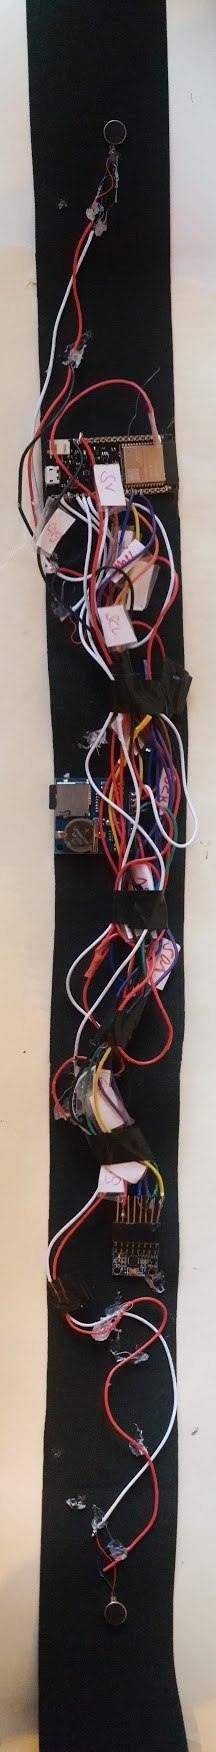
\includegraphics[width=0.14\textwidth]{images/belt.jpg}
    \caption{Belt}
        \label{fig:Belt}
\end{wrapfigure}

After these first attempts I created a simple proof of concept, which is able to read the MPU Data and interpret it to a degree, where I can tell in what direction the user is leaning. So to say, if the broom has fallen or not. This is achieved by simply reading out the accelerometer data and determining the exact position. furthermore, at the beginning of each power-on phase, a baseline reading is done to see the difference in orientation. This baseline reading currently contains of the first second of data. Then a threshold is defined, which is currently defined as follows:

\begin{lstlisting}
 if(baseZacc - (az * 1000) < -150){
       Serial.println("LEANING BACKWARD");
      digitalWrite(BACKWARD, HIGH);
    }else if(baseZacc - az * 1000 > 150){
      Serial.println("LEANING FORWARD");
      digitalWrite(FORWARD, HIGH);
    }
    if(baseYacc - ay * 1000 > 100){
       Serial.println("LEANING RIGHT");
     digitalWrite(RIGHT, HIGH);

    }else if(baseYacc - ay * 1000 < -100){
      
      Serial.println("LEANING LEFT");
      digitalWrite(LEFT, HIGH);
     }
\end{lstlisting}

The baseZacc, baseYacc and baseXacc are the values which was are read in the first second. 

Furthermore, there are four vibrators which vibrate in the direction the "broom is falling", so front, back, left or right. Additionally, the data is also recorded into an SD Card with a time-stamp. All these individual parts are soldered together and fitted into a belt which can be worn, which is displayed in the picture on the right.

The power-source still is outside of the belt, in the form of a \gls{lipo battery} which is simply connected via a micro usb cable.

The data collected has will need to be analysed in-depth. Furthermore, it appears that one single sensor does not offer the needed results or precision to detect posture. The current posture model lacks a lot of information and does not have the quality to give useful information. 

\section{Learnings}

After this first attempts I quickly realised, that connecting all the sensors via cable limited me drastically due to the restrictions of the Wire.h library and the I2C protocol. Due to the addressing issues with the current configuration, some sort of multiplexer, or custom created accelerometers and gyroscopes is needed. Custom parts would currently be way to complicated and multiplexers add unnecessary complexity to the project, I have been looking for another solution. The solution should enable me to scale up the number sensors without back-draws.

Furthermore, the current cable management and hardware complexity will need to be simplified. The current build is much higher than desired and will need to be simplified. Especially since it should be reproductionable.


\addcontentsline{toc}{chapter}{Current Attempt}
\chapter*{Cersion 2}
\label{chap:Technical CHallenges}
\renewcommand{\thesection}{\arabic{section}}
\setcounter{section}{0}

After my first attempts and some discussion with my supervisor i realized that the solution is to distribute the system and send the data wirelessly. This enables me to add additional sensors without having issues with the Wire library. However this increases the cost and complexity of each sensor slightly, since each sensor needs some sort of "brain", which handles the connection and communciation. 
However it reduces the complexity of the construction and the entire solution drasticly since it has single services talking ot each other and not an entier blob of logic. 

\section{Attempt 1}

The communication wase firstly achieved via WIFI since I know the protocol and can get it running swiftly. Also the esp32 I have been using has WIFI natively enabled. 
An issue with wireless communication is the synchronisation of the data flow. To simplify the process and due to lack of knowhow and time to achieve a correct synchronisation I will ignore it, while knowing the data might be timeshifted. 
This might be an issue when visualising and analysing the data, but will be tackled then.

Forthermore for the communication via WIFI a simple "Client Server" protocoll was used which has already been widely implement in ESP32.

Server Client Request: 
\begin{lstlisting}
String clientRequest(String input)
{
  Serial.println(input);
  String response = "\0";
  for (int i = 0; i < NUM_CLIENTS; i++)
  {
    WiFiClient client = server.available();
    client.setTimeout(50);
    if (client) {
      if (client.connected()) {
        client.println(input);
        data = client.readStringUntil('\r');  // received the server's answer
        Serial.println(data);
        if (data != "\0")
        {
          int Index = data.indexOf(':');
        
          CLIENT = data.substring(0, Index);
          ACTION = data.substring(Index + 1);
          Serial.println(data);
   
          if (CLIENT == "ACK")
          {
            response = ACTION;
          }

          //client.flush();
          //data = "\0";
        }
      }else{
        Serial.println("client not connected");
      }
    }
    else{
        Serial.println("client null or false");
      }
  }
\end{lstlisting}

Client Loop:

\begin{lstlisting}
void loop () {
  if (!client.connect(server, 80)) {
    while (WiFi.status() != WL_CONNECTED) {
      Serial.print(".");
      delay(500);
    }
    Serial.print("+");
    delay(100);
    return;
  }
  data = client.readStringUntil('\r');  // received the server's answer
  Serial.println(data);
  if (data != "\0")
  {
    int Index = data.indexOf(':');

    CLIENT = data.substring(0, Index);
    ACTION = data.substring(Index + 1);

    if (CLIENT == CLIENT_NAME)
    {
         client.println("ACK:" + getData());
      
    }else{
        client.println("\0");
    }

    client.flush();
    data = "\0";
  }
}
\end{lstlisting}

The Data will be sent 10 times per second for evaluation purposes. 
However I hope and think this can be reduced, since we hopefully will not need that much data to determine how to usere i positioned. This would enable us to aggregate the data on the devices, which is a benefit only achievable by the current configuration of "Smart-sensors".

The Data is saved onto an SD Card, this works well and enables to analyse de Data afert measuring it for a while. This Concept worked quite well, hovewer it has some major flaws. 

\section{Flaws of Attempt A}

The Idea of saving all the data locally came with the plan to have everything locally which then in a further step could be sent the a smartphone or a laptop without any interent. Maybe with bluetooth or a local hotspot. 

During the development and testing of this concept, it turned out that the client server network was not very stable and it required much more hardware than i woud have liked. 
The Server needed a few modules for it to work.

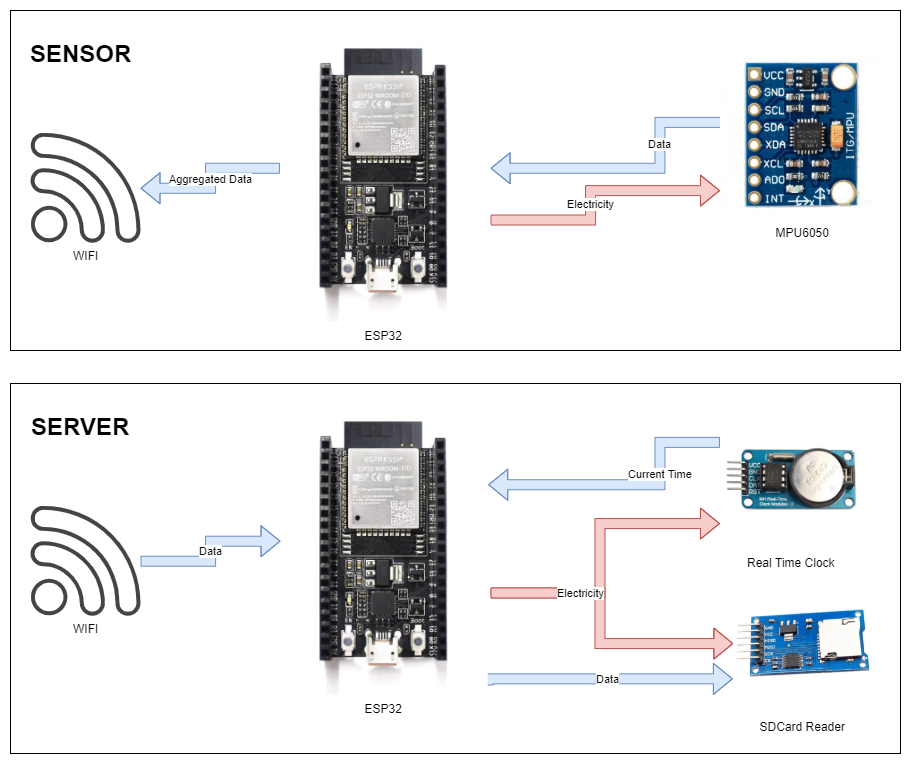
\includegraphics[width=\linewidth]{images/CommunicationDiagrammExplenation.png}

This does not sound like mucht but both of these elementes are quite complex and need to be configured additionally. This felt like quite the hassle and i sonn realized i need to find a new way to communicate.

Beside these technical issues the data transfer during the development phase, where bluetooth or hotspot was avaialble was quite awkward since the device need to be stopped and the data needed to be analysed in a spereate step. 


\begin{center}
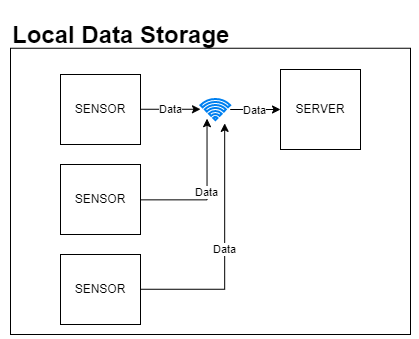
\includegraphics[width=0.5\textwidth]{images/CommunicationDiagrammLocal.png}
 \end{center}
After working with it for a while I tried to find a much simpler way, which is closer to the goal of a simple and affordable sensor set. To Tackle the issues with the client server network i first thought of using a simple http request, which would have a bit more overhead but would be more stable. This however didn't feel right and I realized that the solution, was something I already was quite familiar with. A simple MQTT Broker. 



\section{Atempt B}

After this first attempt i knew how to handle the message and date from the sensors which helped greatly. 
The Communication in my new attempt was handled with a simple MQTT Broker, which can be setup for free within seconds. For my endeavours I used cloudmqtt.com which is completly free and easy to apply. 


\begin{center}
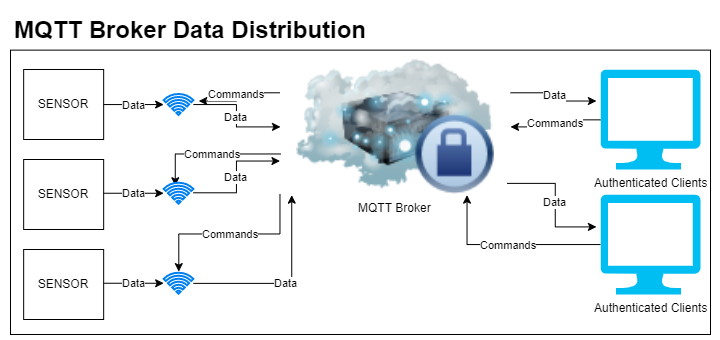
\includegraphics[width=0.8\textwidth]{images/CommunicationDiagrammMQTT.png}
\end{center}
MQTT uses a simple publish subscribe protocoll which I have already implemented a few times.
Below you see the whole setup and loop code, which is almost readable thanks to helper functions:
\begin{lstlisting}
void setup() {
  Serial.begin(115200);
  Wire.begin();
  USERID = getRegisterdUserid();
  setupMPU();
  setupWifi();
  client.setServer(mqtt_server, mqtt_port);
  client.setCallback(callback);

  strcpy(fullsubtopic, TOPIC); 
  strcat(fullsubtopic, USERID);
  strcat(fullsubtopic, SUB);
  
  strcpy(fullpubtopic, TOPIC); 
  strcat(fullpubtopic, USERID);
  //strcat(fullpubtopic, PUB);
  
  while (!client.connected()) {
   reconnect();
  }
  startMillis = millis(); 
  getData();
}

void loop () {
  client.loop();
  currentMillis = millis();  //get the current "time" (actually the number of milliseconds since the program started)
  if (currentMillis - startMillis >= period)  //test whether the period has elapsed
  {
    Serial.println("trying to send");
    char * message = getMessage();
    publish(message);
    Serial.println(message);
    startMillis = currentMillis;  //IMPORTANT to save the start time of the current LED state.
  }
 getData();
 }
\end{lstlisting}

This loop collected the data into an average in "getData()" function
\begin{lstlisting}
void getData(){
  if(readByte(MPU6050_ADDRESS, INT_STATUS) & 0x01) {  // check if data ready interrupt
    readAccelData(accelCount);  // Read the x/y/z adc values
    getAres();
    ax = (float)accelCount[0]*aRes - accelBias[0];  // get actual g value, this depends on scale being set
    ay = (float)accelCount[1]*aRes - accelBias[1];   
    az = (float)accelCount[2]*aRes - accelBias[2];  
    readGyroData(gyroCount);  // Read the x/y/z adc values
    getGres();
    gx = (float)gyroCount[0]*gRes - gyroBias[0];  // get actual gyro value, this depends on scale being set
    gy = (float)gyroCount[1]*gRes - gyroBias[1];  
    gz = (float)gyroCount[2]*gRes - gyroBias[2];  
    tempCount = readTempData();  // Read the x/y/z adc values
    temperature = ((float) tempCount) / 340. + 36.53; // Temperature in degrees Centigrade
 
    accelVal[0] = ax;
    accelVal[1] = ay;
    accelVal[2] = az;
    gyroVal[0] = gx;
    gyroVal[1] = gy;
    gyroVal[2] = gz;
    setAvg();
    
   }
}
void setAvg(){
    for (int i = 0; i < 3; i++){
      avgAccelVal[i] = (avgAccelVal[i] + accelVal[i])/2;
      avgGyroVal[i] = (avgGyroVal[i] + gyroVal[i])/2;
  }
}
\end{lstlisting}
 and created a json from the collected data in the "getMessage()" function which was sent every second: 
\begin{lstlisting}
char* getMessage(){
  char* a = "{ \"id\": \"";
  char* b = "\", \"acc\":[";
  char* c= "], \"gyro\":[";
  char* d= "]}"; 
  char accelbuff[64];
  char gyrobuff[64];
  Serial.println("loading data to buffers");
  char* loc = accelbuff;
   size_t tempLen;
   int i = 0;
   for(i = 0; i < DIM(avgAccelVal)-1; ++i)
    {
        snprintf(loc, 12, "%f,", avgAccelVal[i]);
        tempLen = strlen(loc);
        loc += tempLen;
    }
   snprintf(loc, 12, "%f", avgAccelVal[i+1]);
   tempLen = strlen(loc);
   loc += tempLen;
   loc = gyrobuff;
   for(i = 0; i < DIM(avgGyroVal)-1; ++i)
    {
        snprintf(loc, 12, "%f,", avgGyroVal[i]);
        tempLen = strlen(loc);
        loc += tempLen;
    }
  snprintf(loc, 12, "%f", avgGyroVal[i+1]);
  tempLen = strlen(loc);
  loc += tempLen;
  strcpy(messagebuffer, a ); 
  strcat(messagebuffer, DEVICEID);
  strcat(messagebuffer, b);
  strcat(messagebuffer, accelbuff);
  strcat(messagebuffer, c);
  strcat(messagebuffer, gyrobuff);
  strcat(messagebuffer, d);
  return messagebuffer;
}
\end{lstlisting}
As you can see the creation of the message, was almost the most complex part of the implementation. This was due to the fact, that the mqtt Library could not handle "arduino" Strings and therefored need char* which are a mess to work with. Nontheless after some tinkering i finally managed to get a nice JSON message over the MQTT Broker: 
\begin{lstlisting}
{ 
    "id": "SENSOR-XSZ", 
    "acc":[-0.003835,0.001486,0.056012],
    "gyro":[0.056012,0.240598,0.038814]
}
\end{lstlisting}

Additionally I enabled all devices to be calibrated remotely. This since when i put these devices on I will ned to calibrate them after they are set in position. This is quite a simple task with MQTT since the clients can simply subscribe to a topic, from which they get messages: 

\begin{lstlisting}
void callback(char* topic, byte* message, unsigned int length) {
  Serial.print("Message arrived on topic: ");
  Serial.print(topic);
  Serial.print(". Message: ");
  String command;
  
  for (int i = 0; i < length; i++) {
    Serial.print((char)message[i]);
    command += (char)message[i];
  }
  if(command == "calibrate"){
    calibrateMPU6050(gyroBias, accelBias); // Calibrate gyro and accelerometers, load biases in bias registers  
    initMPU6050(); 
    Serial.println("MPU6050 initialized for active data mode....");
  }
}
\end{lstlisting}
This callback gets registered when connecting to the mqtt broker.



\subsection{Benefits Version B}

The Benefint of managing the messages via a MQTT Broker was that I could get the messages and work with them from any device with an Internet connection. This means that any calculation heavy tasks can be done from a "real" computer which handles these much better. 

This also enabled me to visualize and analyze the data in realtime which made it much easier. 

Furthermore it also achieves the goal of being cheap and affordable. Since we now only need MPU6050 and microntrollers to send the data and this can be setup much easier than with an ESP32 "server".

This also means that there does not need to be any more logic on the devices itself since everyhting can be done from a Computer. Maybe some sort of vibration device will be added which however also can be activated via the MQTT Broker. 

The Fact that these sensors now can simply send data without knowing where they are or what exactly they are measuring might open quite a lot of doors. I will get further into that in a later chapter.

\subsection{Backdraws Version B}

The Obvious backdraw is, that the sensors need to have a constant interent connection. This is obviously not great, especially when we try to develop something for an every usage since we are somewhat bound to a single place. 

Furthermore if used as a product, these sensors would need to be registered first bevor usage, this does increase complexity for a first usage however simplifes setup greatly.


\section{Identifying Posture}

The biggest hurdle, was and still is identifying and correctly analysing the data. I have had several different approaches on how to interpret and visualise the data. During my first attempt (Attempt A) i tried to visualised the data in two ways, with Python and Power BI.

Firstly I transformed the data into a \acrshort{csv} (\gls{CSV}). CSV is a commonly used format viable for many different applications

According to the datasheet of the MPU6050 the collected data is "g-force". The accelerometer measure in mg and the gyroscope in \degree/s. 

\begin{figure}[h]
\begin{center}
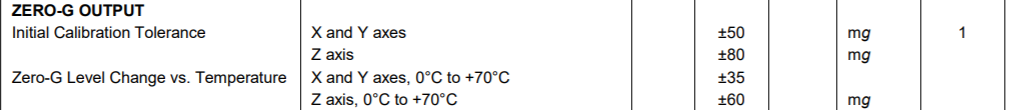
\includegraphics[width=\linewidth]{images/MPU6050_DATA.png}
  \end{center}
  \caption{MPU Datasheet}
  \label{fig:MPUDatasheet}
\end{figure}

The entire documentation can be found online \cite{MPU6000D59:online}.

\subsection{Visualising with Python}

I tried to visualise the data using \gls{Python} since it was recommended on a few forums and seamed to be feasible for this task. It actually did work quite well and I have achieved within 2 Days with Python. I have never worked with python before and was happy that I managed to use and apply it within days. 

\begin{figure}[h!]
\begin{center}
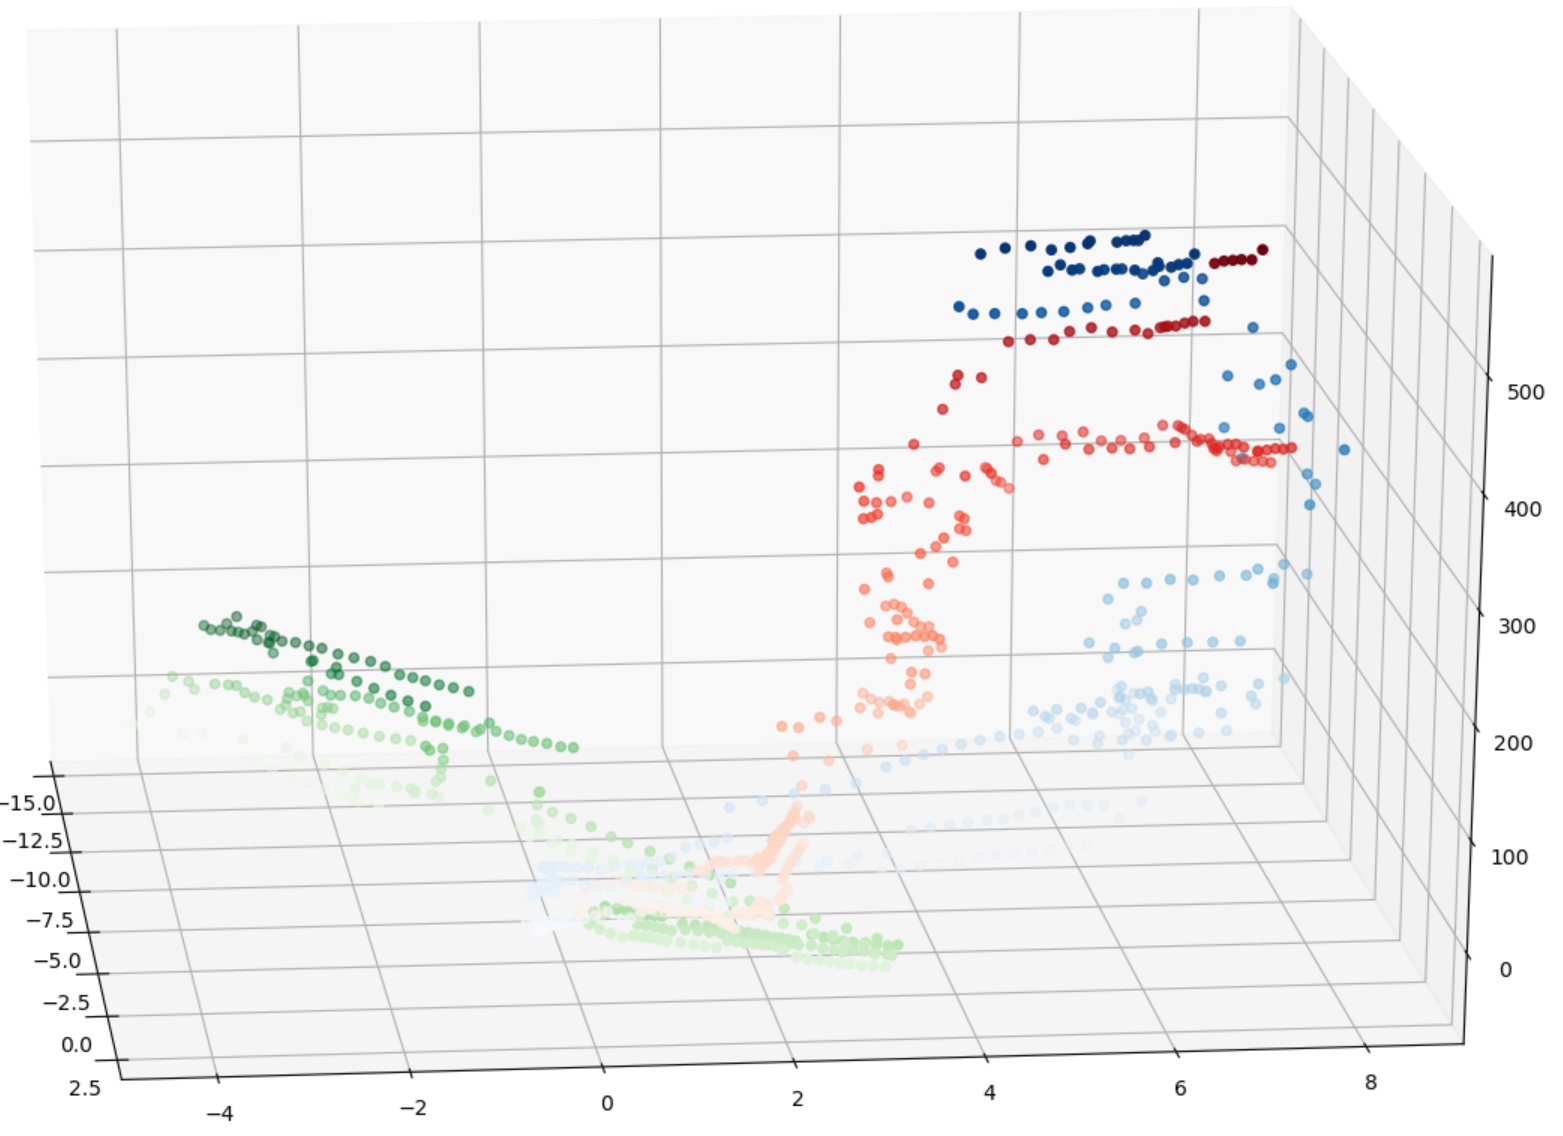
\includegraphics[width=0.6\linewidth]{images/PyVisualisation.png}
  \end{center}
  \caption{Python Visualisation}
  \label{fig:PythonVisualisation}
\end{figure}

Visualised you see my first attempt in figure \ref{fig:PythonVisualisation}, showing movement of 3 sensors with the data of the accelerometers. The sensors were attached to my shirt with scotch. This is not a perfect solution, which is visible in the different orientation of the green dots. 

Here I tried to add up the movement from the accelerometers to see how this stacks up. The Data was not very helpful and i tried to anime the accelerometer data directly to see how it changes, this was a bit clearer but still very hard to interpret since it was static data. 

To visualise I used numpy and matplotlib which are quite handy but still took some time the get used to.
The data was simple display on a grapth (ax) from np arrays:

\begin{lstlisting}
ax.scatter3D(XSXAcc[:,0],XSXAcc[:,1],XSXAcc[:,2], c=XSXAcc[:,2], cmap='Reds')
ax.scatter3D(XSYAcc[:,0],XSYAcc[:,1],XSYAcc[:,2], c=XSYAcc[:,2], cmap='Blues')
ax.scatter3D(XSZAcc[:,0],XSZAcc[:,1],XSZAcc[:,2], c=XSZAcc[:,2], cmap='Greens')
\end{lstlisting}

\subsection{Visualising with Power BI}

\gls{Power BI} is a very powerful tool which I was already used to, since we used it at work to visualise project data and quality gates. Therefore it was much easier for me to visualise the data.

During different attempts of visualising the data i realised, it made sense to visualise it with a 2d graph, since the three dimensional visualisation did not offer any real benefits. Furthermore during this visualisation I also quickly saw, that the data collected had to be incorrect, since the accelerometer should never fluctuate as much as it did. The error was in my code and was quickly fixed, however I still had issues making conclusions from this static data.

\begin{figure}[h]
\begin{center}
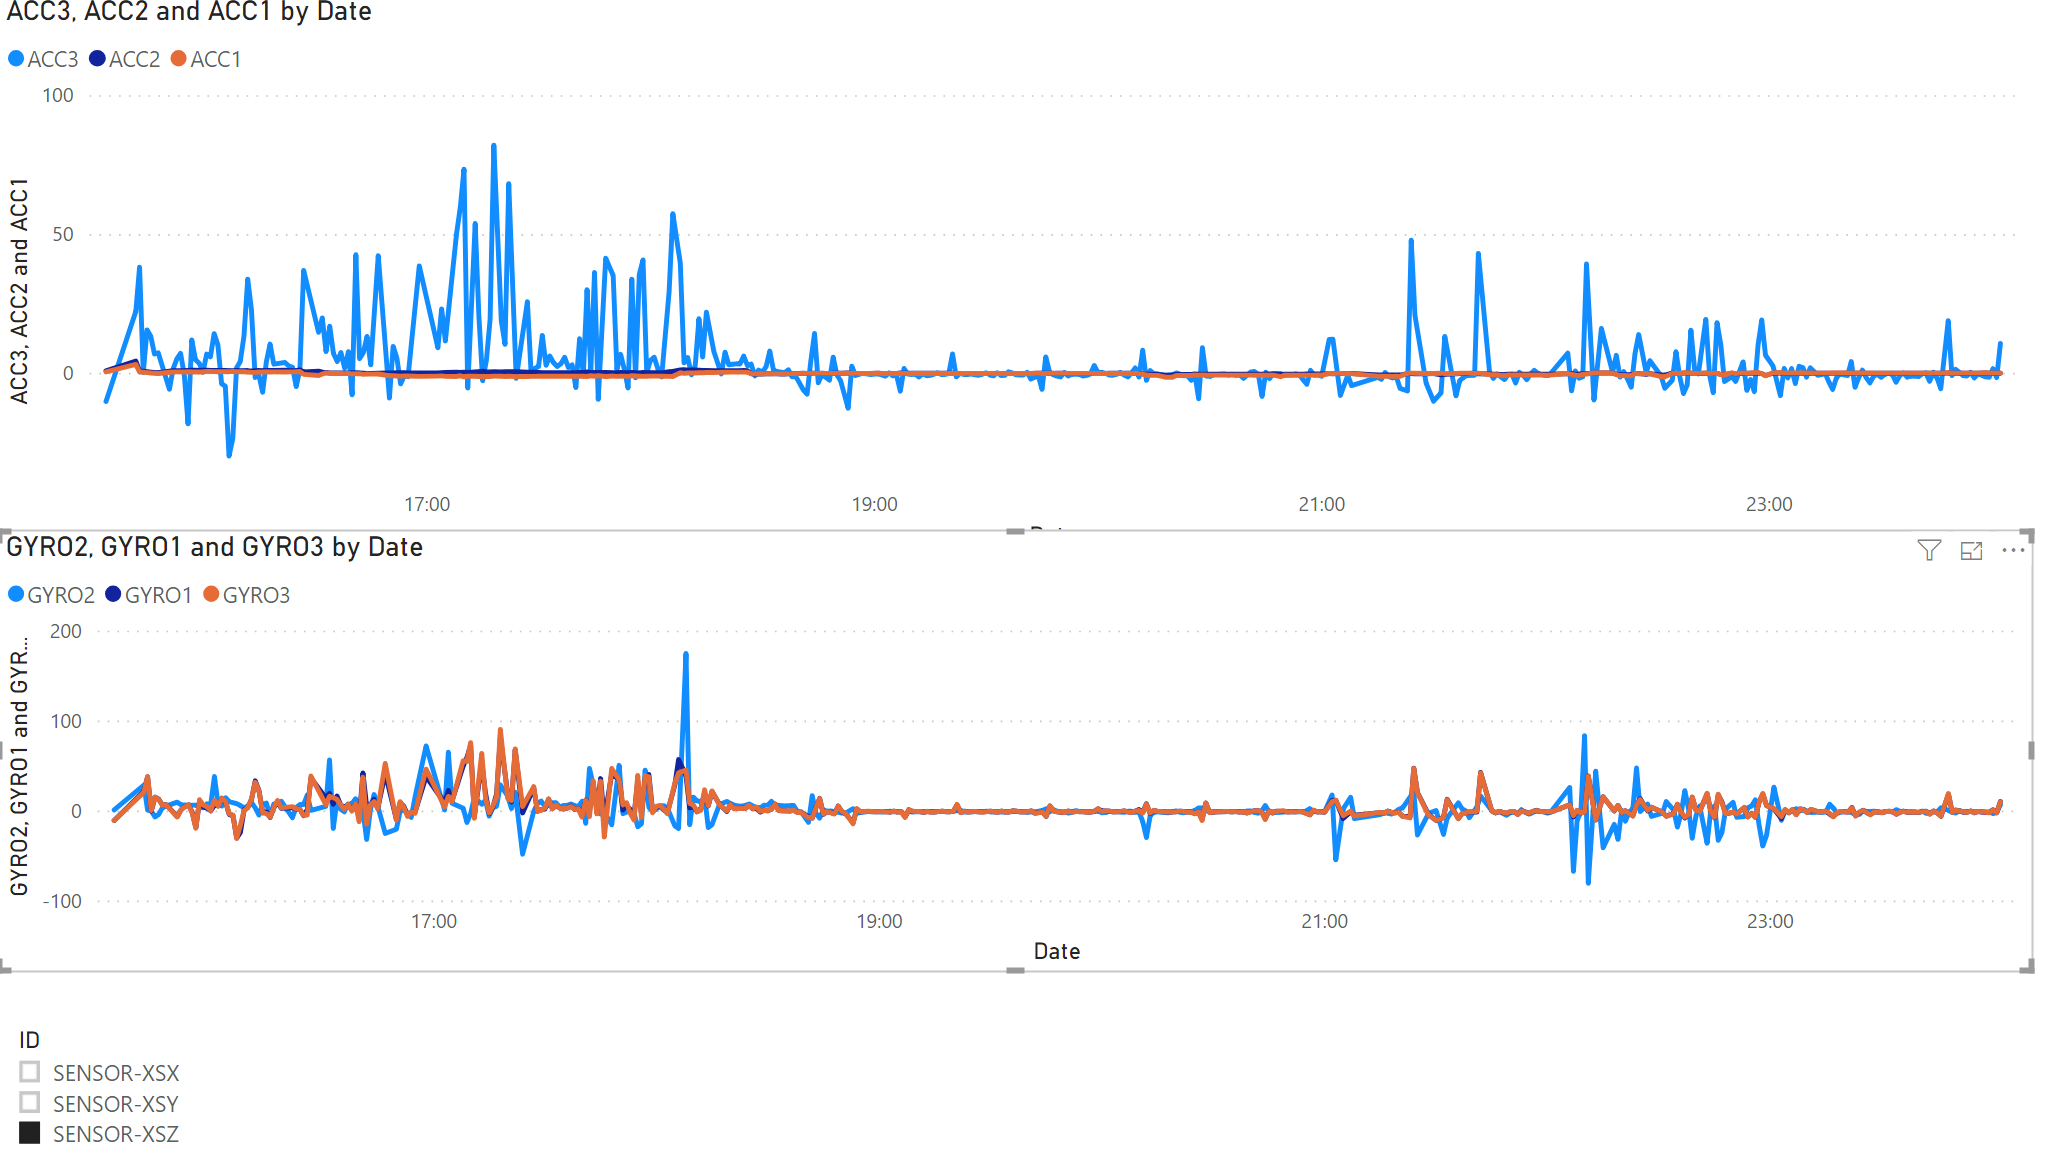
\includegraphics[width=0.7\linewidth]{images/PowerBIVisualisiation.png}
  \end{center}
  \caption{Power BI Visualisation}
  \label{fig:PowerBIVisualisation}
\end{figure}

\newpage



\addcontentsline{toc}{chapter}{Results}
\chapter*{Results}
\label{chap:Results}
\setcounter{section}{0}

During my thesis I learnt a lot about posture and sensors and achieved a great base for further projects and continuing this journey. I definitely did not create a finished product, however, this was never the goal of this projects. Nonetheless I achieved a view goals which I have listed below.

\section{Quick Summary}

As a quick summary of all goals and learning, it can be said, that a minimum of two Sensors are needed from which one must be positioned on the lower back and one on the upper back. Due to this positioning it is nearly impossible to change posture without the sensors to detect it. Additional sensor would help improving precision and fine tuning however, are not necessary. The right posture is defined by the user itself and not defined by the software. A "global" correct position could be set using this setup, however, was found not to be useful or recommendable. \cite{SitUpSt77:online} Additionally the user can also set posture he would like to avoid.

The user gets a vibration feedback from the sensor, and a visual feedback from the software when the set posture goal is not met. The analysis of these value is done with the median of a 10 second measurement, since a quicker refresh rate does not offer any real benefit and it reduces useless vibrations due to hectic movement.

\section{Achieved Goals}

In the evolution of this project, I simplified the data transfer and created a first definition how the sensors can be "dumb". Thanks to this the "sensor packets" got much simpler and need much less soldering. I was able to move all logic from the devices to any language or system desired without losing any significant response time. 

\begin{figure}[h]
  \begin{center}
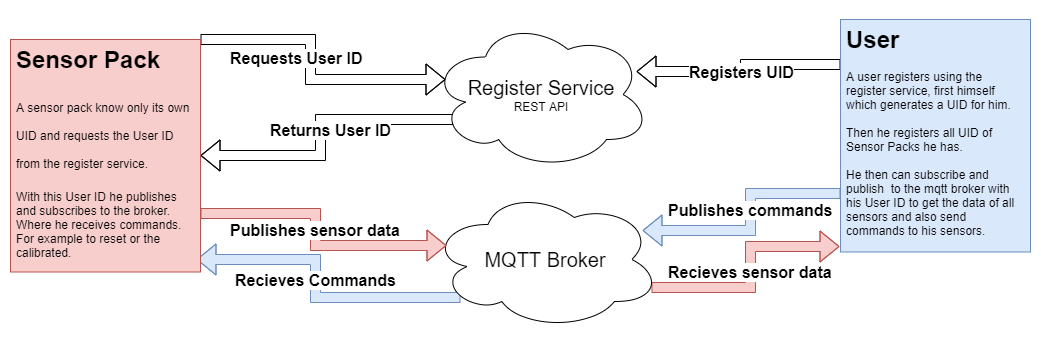
\includegraphics[width=\textwidth]{images/DumbSensor.png}
  \end{center}
  \caption{Sensor workflow}
  \label{fig:SensorWorkflow}
\end{figure}

With the flow displayed above, in figure \ref{fig:SensorWorkflow}, the sensors can all have the same logic and only need  a unique id to be identified and no further setup. It needs to be noted, that the register service was not fully implemented for this thesis, however, it was mocked. This since it does not add any value to the thesis or the goals of this thesis.

Thanks to these adjustments and improvements during this project, live data visualisation was achieved. This is on one hand a cool feature however, it also simplifies the analysis and understanding of the collected data vastly. It helped me really understand the data and transfer it to a simple posture model. Which then enabled me to visualise the positioning of the sensors and the posture. Additionally thanks to my better understanding of the sensor data and collected data, how it can be used to model posture and my experience gained through the first versions, I know how a single self contained sensor pack could be implemented. This would be easier to user however, much more restricted. 

Also due to the abstraction of logic, it became much easier working with the data and I think it also improved the re-usability, since logic can be implemented in any language desired and is not restricted to c++.

\subsection{Improving Posture}

Posture is quite a difficult topic, and I would be overselling, when writing, that I can improve posture with this concept. Since I have not many long term tests or studies I cannot confirm or deny that. however, what I can do is read about good posture and how it can be improved and try to follow these principals. This is exactly what I did. According to the paper ""Sit Up Straight": Time to Re-evaluate" \cite{SitUpSt77:online} the right posture is not globally given or can be set for every person on this planet. 

In the following graphics the writer of the paper summarised their findings:
\begin{figure}[h]
  \begin{center}
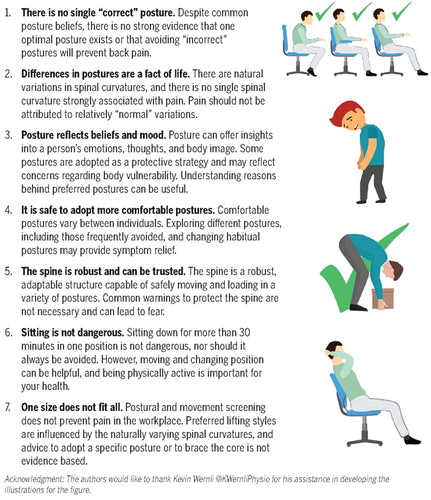
\includegraphics[width=0.7\textwidth]{images/jospt-562-fig001.jpg}
  \end{center}
  \caption{Posture Study \cite{SitUpSt77:online}}
  \label{fig:Posture Study}
\end{figure}

Most interesting for me are the first two points, which indicate that my posture module must be agile and adjustable to each user individually. This is also why I did not set a default goal, which a user must try to achieve. Each user can set their own goals. According to my understanding, it is the only way to safely and individually improve posture.This approach still has some risks and might lead to uncertainties with users. 
The user might not know what a good posture is and train a wrong posture or be afraid of training a wrong posture and not using this concept. This could be tackled by contacting a professional for a first input and an initial setup of the device.

\subsection{Being Open source}

All the code created for this project will be released on my git repository soon. An introduction and explanation will be available as well, including a list of parts needed to build the same devices. The code and all the documentation will be available as soon, as the code has reached a standard and cleanliness I can get behind. The Goal is to accomplish this at the time of submitting this paper.

\section{Open Goals}

From my goal of creating a simple affordable solution to improve posture, a lot has been achieved. Nonetheless I did not create the type of solution I first had in mind. I would not consider this a problem, since the current solution is much more flexible. However, my first goal, which I tried to achieve in the first version, was a single contained unit which achieves posture improvements. This would be possible with the know-how I have now and will also be kept as a long term goal. however, I feel that much more can be achieved with the distributed network I have implemented currently. 

Currently this sensor network is a simple proof of concept and I will definitely need to implemented some things I have mocked to create a usable and user friendly product.  The Register service would need to be implmented and also the web app needs a lot more work. It is currently not very user friendly and only configured to work with my 3 sensors. 

Furthermore, when the register service is available the sensors need more work, to enable a complete self provisioning, since currently the network connection is hard coded. This is not very interesting or hard since it has been implemented multiple times (https://www.arduino.cc/en/Reference/WiFiNINABeginProvision), therefore I left it out. 

Security also is an issue that was only thought of however, not implemented correctly. Currently the MQTT Broker is a secured by credentials however, these also are hard-coded and would need to be different for every user. MQTT offers this possibility and also encrypts the messages.

Lastly the size of the sensor packets is far from optimal and could be drastically reduced by creating a single plate with all logic withing. This will not be a goal that I will tackles soon, since this would be the last step of creating such a "product".


\section{Learnings}

Firstly I understood how the MPU6050 sensor works with the wire library, learned much more about Arduino coding. I also learned the communication with other sensors and actors, like the SD card reader or the real time clock. Furthermore, I learned what to be aware of when working with micro-controllers, how to setup a simple client server network with minimal resources. All of this was necessary to achieve a simplified and usable sensor pack. 
To position the sensor pack I had to test multiple positioning and discuss with a physiotherapist what a useful position would be. According to my understanding the current optimal position would be directly on the spine, and at least two sensors, one on the upper and one on the lower back. Every additional sensor improves the precision of the posture model. 

Additionally the learning will be applicable on the first version of the project. As mentioned two sensors are necessary for a useful analysis of posture, nonetheless with the current know-how I know that some measurements are still possible with a single sensor unit. it will need to be analysed with a long-term test, how much information is lost when using a single sensor and whether the lost information is critical for a daily wearer.

To understand the positioning I also had to understand what posture is. This was only possible through research and unfortunately this know how is still very limited.

\section{Project Management}

In the beginning of the Project a lot of goals were defined. These goals were tagged as necessary or optional. however, the goals changed greatly during the thesis, since new ideas emerged. Non-theless the primary necessary goals, stayed the same and are defined as follows: 
\renewcommand{\thetable}{\arabic{table}}
\begin{center}
\begin{table}[h!]
\begin{tabular}{|p{9cm}|p{3cm}|p{3cm}|}
  \hline
 \textbf{Goal} &\textbf{ Planned  } &\textbf{ Completed By } \\ 
  \hline
 Communication between ESP32 and Sensors & July 2019 & July 2019   \\  
 \hline
 Collect the data  & August 2019  & August 2019   \\  
  \hline
 Enable multi Sensor communication (Client, Server) & September 2019 & September 2019   \\ 
  \hline
 Enable multi Sensor communication (MQTT) & - & October 2019   \\ 
  \hline
 Visualise the data & October 2019 & November 2019   \\  
  \hline
 Real time visualisation (WebApp) & - & December 2019   \\  
   \hline
 Sensor position and amount & November 2019 & December 2019   \\ 
  \hline
 Identify posture & November 2019 & December 2019   \\  
  \hline
 Visualise posture & December 2019 &  December 2019 \\    
   \hline
 Visualise and communicate wrong posture & December 2019& January 2020 \\    
  \hline
\end{tabular}
\caption{Planned and unplanned goals}
\label{table:1}
\end{table}
\end{center}

\subsection{Technical implementation later than expected}

Originally it was planned to have everything technical, software and hardware, done in the beginning of December. however, due to the MQTT data transfer implementation and the visualisation of the data with a web app a lot of the work got done later than expected. however, this was manageable since a time buffer was planned in the beginning. Three weeks of holidays in December were planned in the beginning of the project to ensure a certain and non-hectical finish of the implementation. As visible in the table, this three weeks were used and were definitely necessary. 

\addcontentsline{toc}{chapter}{Prospects}
\chapter*{Prospects}
\label{chap:Porspects}
\setcounter{section}{0}

As mentioned much more has to be achieved, even so, a great base was made with which a lot can be achieved. 

\section{The Next Steps}

The project is not over for me, I see a lot of potential. Theses sensors might have a much wider use case than expected and with my current know-how and more time I might be able to measure more than posture. My partner is a physiotherapist and already had some great ides where these sensors might be used. For example to measure bending of knees and other joints. 

Another quite ambitious goal is to visualise movement with the sensors. I am unsure if this is a possibility since the drift of the measurement could be drastic, however this is something I will definitely try to implement, sine if it is possible would open a lot of opportunities.

A goal which is most likely achievable and I would consider a great improvement is adding an additional sensor as a reference point. This would enable users to wear and track posture even when working in a moving environment. This is probably quite hard to calculate out the movement especially due to synchronisation and latency which I was able to mostly ignore during this project.

Furthermore I will also try out other accelemoters and gyrscopes to determine precision and what would be optimal for my use case. This was not considered, since the MPU6050 does offer enough precision and comparing sensors requires a lot of know-how and time.


\cleardoublepage
\phantomsection 
\addcontentsline{toc}{chapter}{Declaration of authorship}
\chapter*{Declaration of primary authorship}
\label{chap:declaration_authorship}

\vspace*{10mm} 

I hereby confirm that I  have written this thesis independently and without using other sources and resources than those specified in the bibliography. All text passages which were not written by me are marked as quotations and provided with the exact indication of its origin. 

\vspace{15mm}

\begin{tabbing}
xxxxxxxxxxxxxxxxxxxxxxxxxxxxxx\=xxxxxxxxxxxxxxxxxxxxxxxxxxxxxx\=xxxxxxxxxxxxxxxxxxxxxxxxxxxxxx\kill
Place, Date:		\> Ostermundigen, \versiondate \\ \\ 
Last Name/s, First Name/s:	\> Gabriel Frischknecht 	 \\ \\ \\ \\ 
Signature/s:	\> ......................................\> \\
\end{tabbing}

%---------------------------------------------------------------------------
% Glossary
\addcontentsline{toc}{chapter}{Acronyms}
\printglossary[type=\acronymtype]
\addcontentsline{toc}{chapter}{Glossary}
\printglossary

%---------------------------------------------------------------------------

% Bibliography
%---------------------------------------------------------------------------
\cleardoublepage
\phantomsection 
\addcontentsline{toc}{chapter}{Bibliography}
\bibliographystyle{IEEEtranS}
\bibliography{database/bibliography}{}
%---------------------------------------------------------------------------

% Listings
%---------------------------------------------------------------------------
\cleardoublepage
\phantomsection 
\addcontentsline{toc}{chapter}{List of figures}
\listoffigures
\addcontentsline{toc}{chapter}{List of tables}
\listoftables
\end{document}

